\section{Results}
\label{sec:Res}

% ----------------------------------------------------------------------- %
% ----------------------------------------------------------------------- %
\subsection{Feasibility of estimations}
\label{sec:feasest}

% Alternative section title: General estimation results







% NOTES:
% - 1) address feasibility of estimations for each estimator
% - 2) give general overview about estimation results (see Breidenbach) before going into more detail
%
%








\newpage
% ----------------------------------------------------------------------- %
% ----------------------------------------------------------------------- %
\subsection{Estimation accuracies}
\label{sec:esterr}













\begin{figure}[H]
	\centering
	\resizebox{1\hsize}{!}{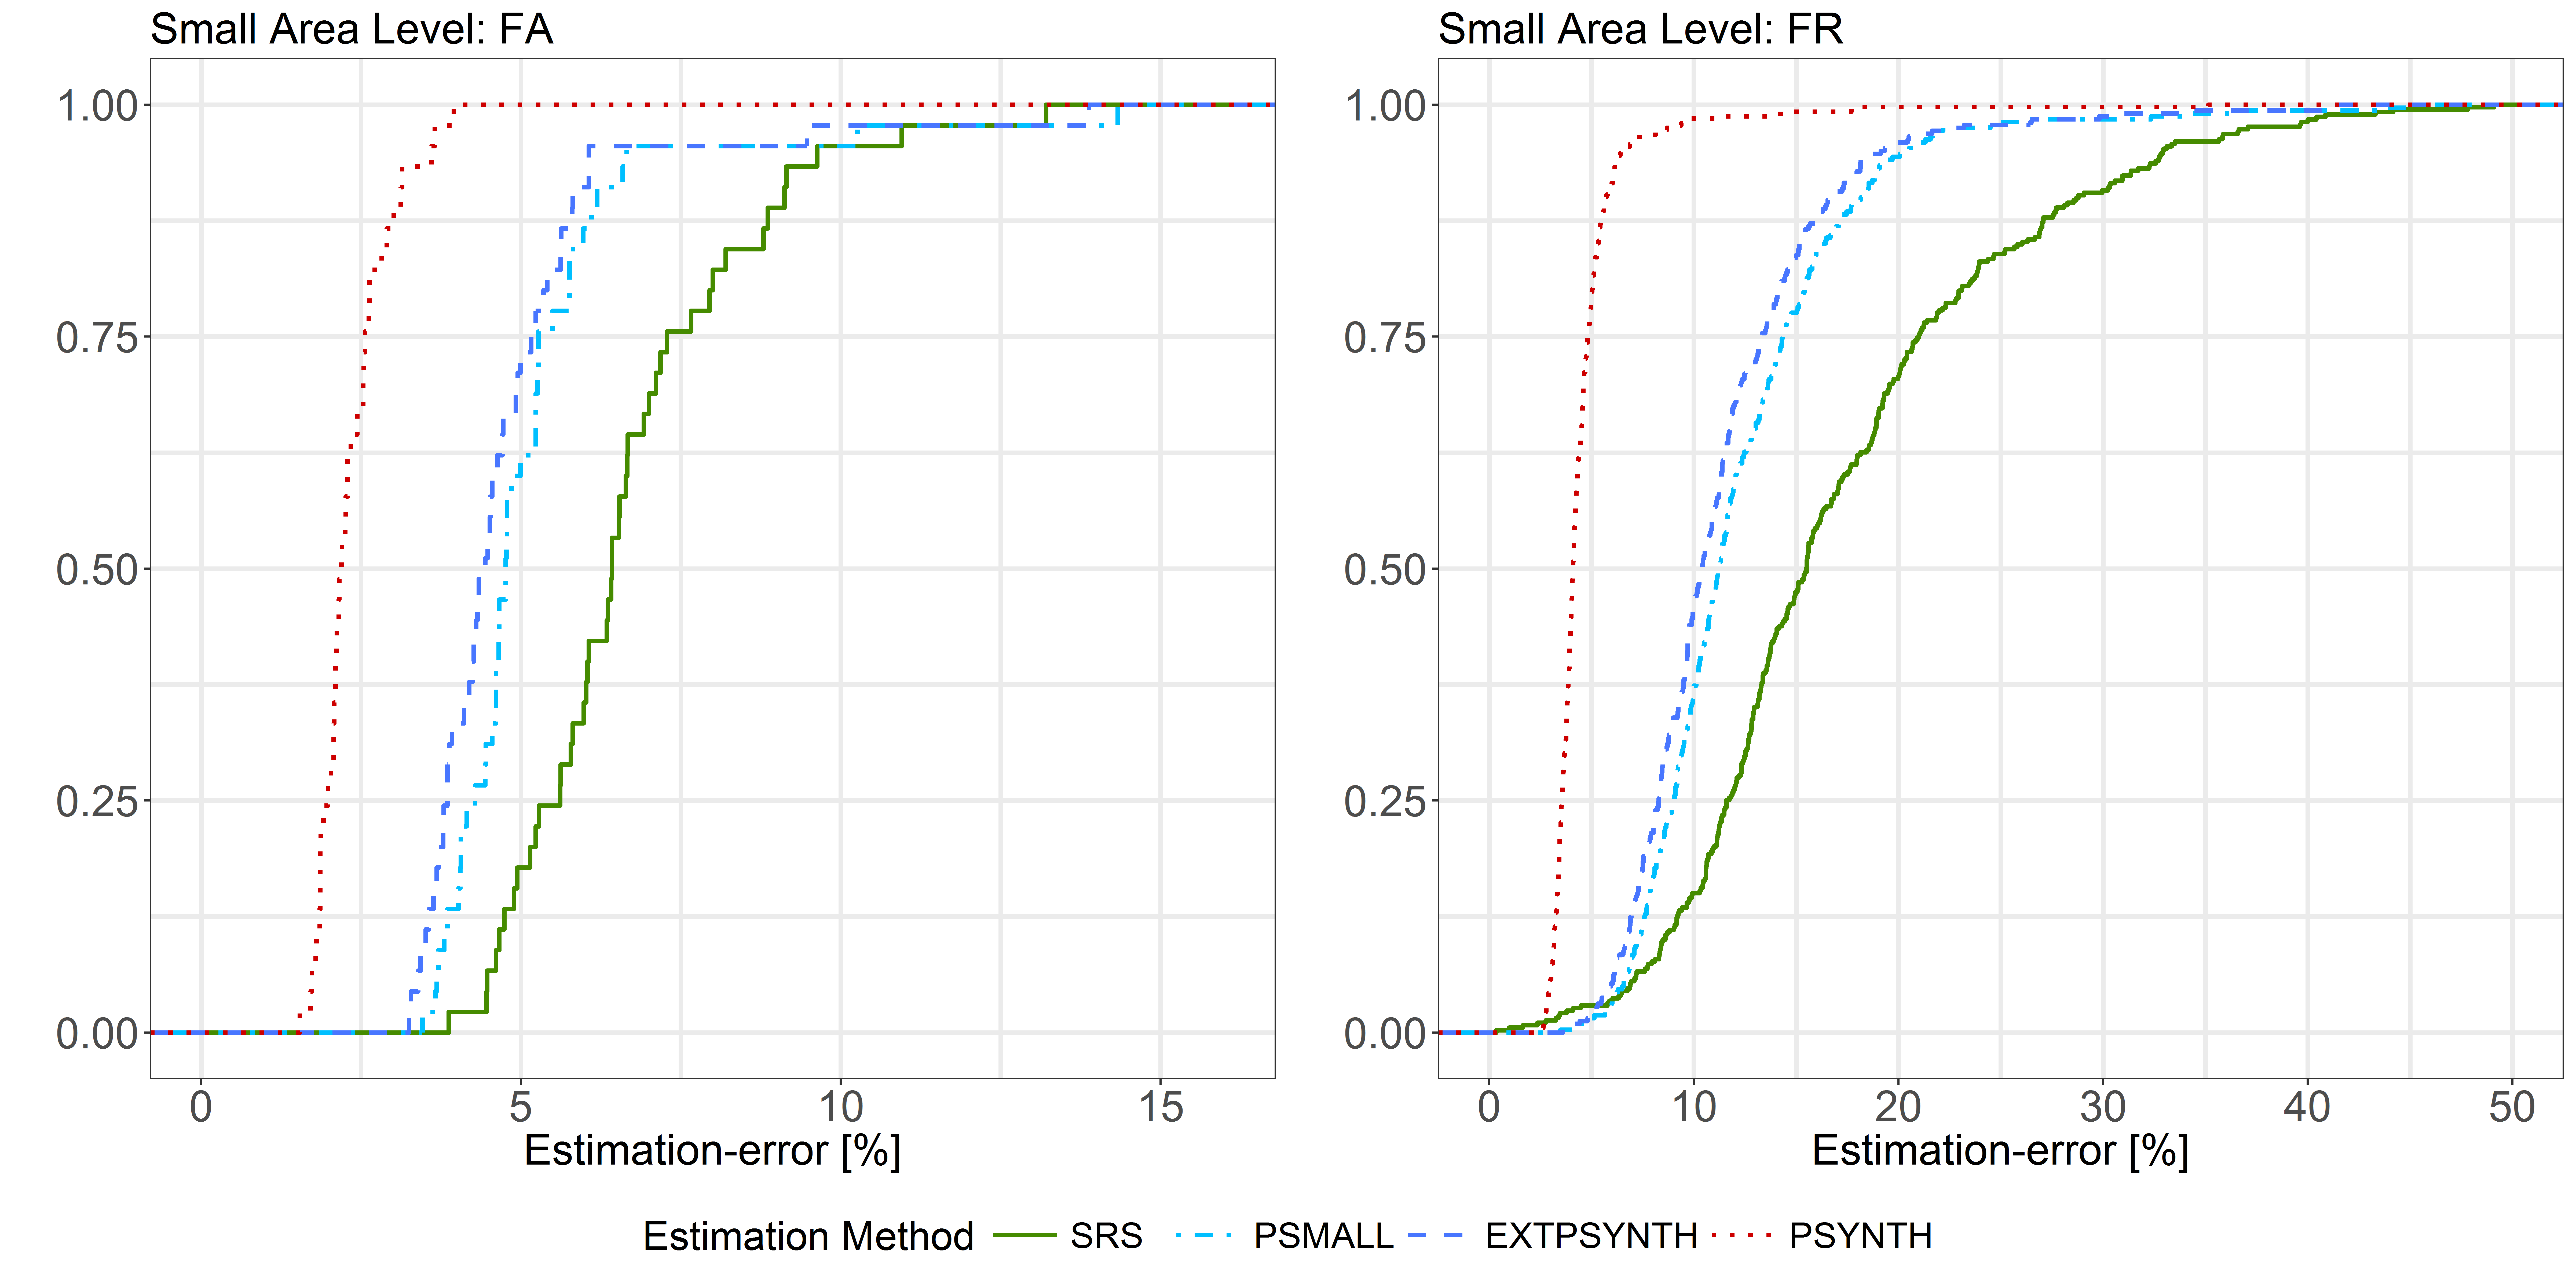
\includegraphics{fig/error_distr_foa_fu.png}}
	\caption{Cumulative distribution of estimation errors under the simple random sampling (SRS), the pseudo small (PSMALL), the extended pseudo synthetic (EXTPSYNTH) and the pseudo synthetic (SYNTH) estimator. \textit{Left}: Results for the 45 FA units. \textit{Right}: Results for the 388 (SRS), 321 (PSMALL / EXTPSYNTH) and 403 (PSYNTH) FR units.}
	\label{fig:disterrors}
\end{figure}



\newpage
% ----------------------------------------------------------------------- %
% ----------------------------------------------------------------------- %
\subsection{Gain and Relative Efficiency}
\label{sec:gain_releff}



















\begin{figure}[H]
	\centering
	\resizebox{0.7\hsize}{!}{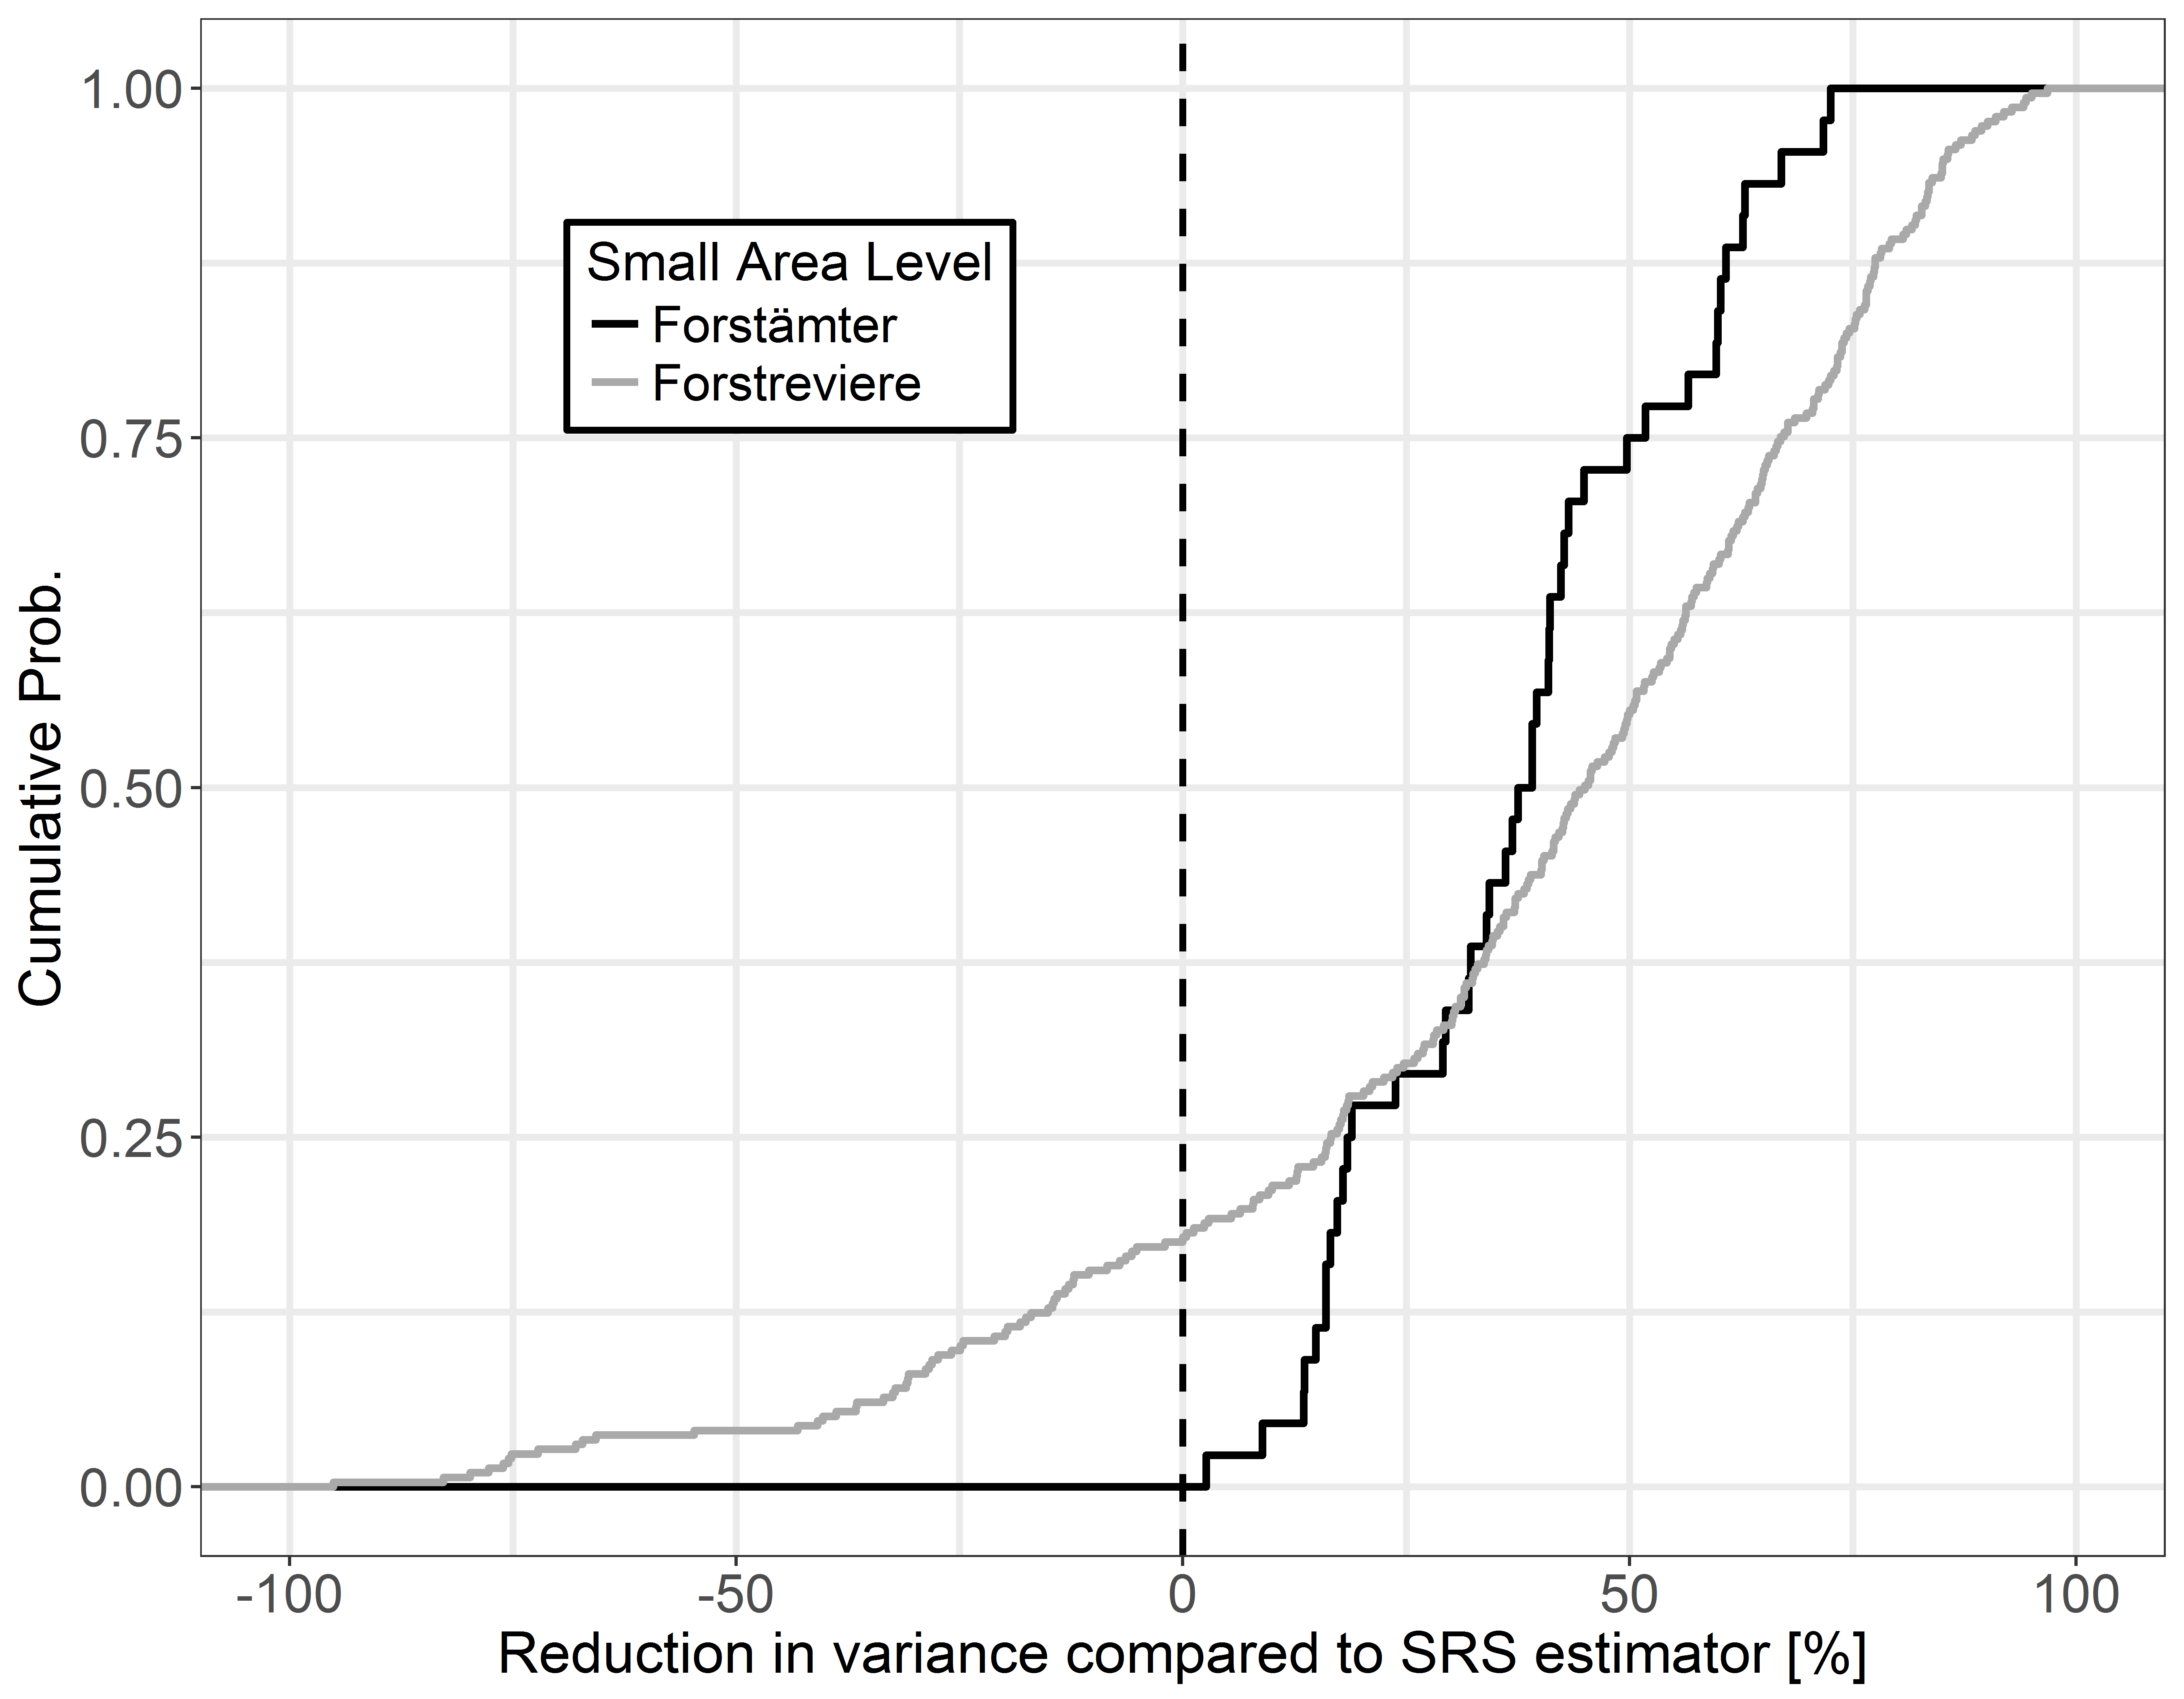
\includegraphics{fig/compare_onephase_psmall.png}}
	\caption{Cumulative distribution of variance reduction by the PSMALL compared to the SRS estimator for the  45 FA and 321 FR units.}
	\label{fig:gain}
\end{figure}





\begin{figure}[H]
	\centering
	\resizebox{0.7\hsize}{!}{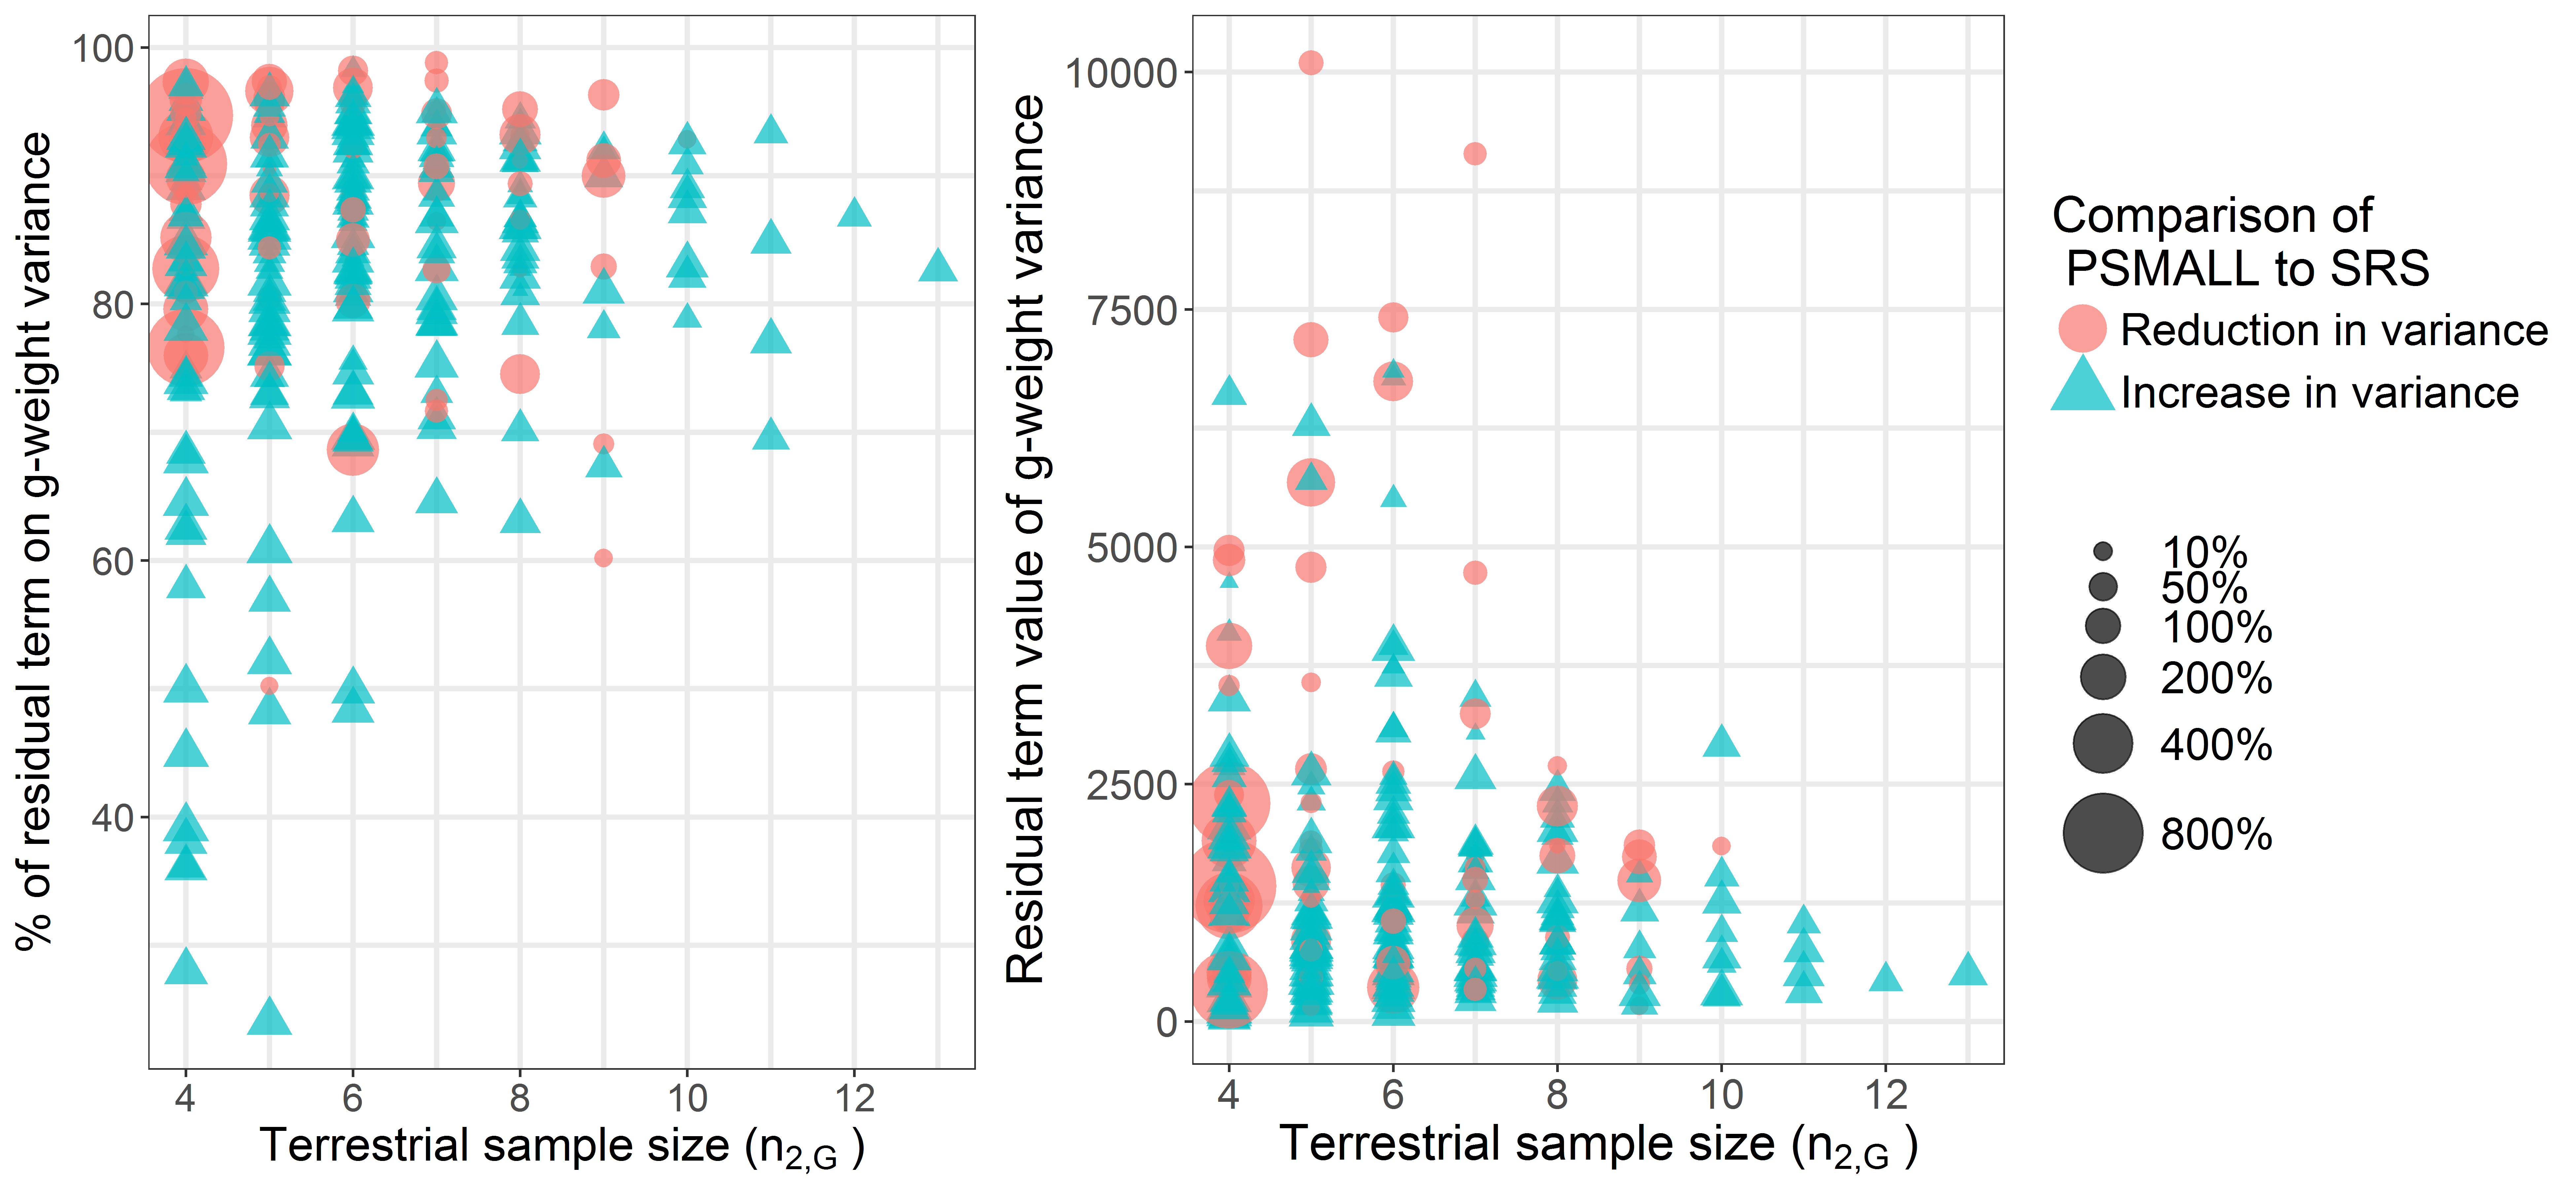
\includegraphics{fig/eval_2phase_fail.png}}
	\caption{}
	\label{fig:fail}
\end{figure}





\newpage
% ----------------------------------------------------------------------- %
% ----------------------------------------------------------------------- %
\subsection{Comparison of PSMALL and EXTPSYNTH}
\label{sec:comp}
















\begin{figure}[H]
	\centering
	\resizebox{1\hsize}{!}{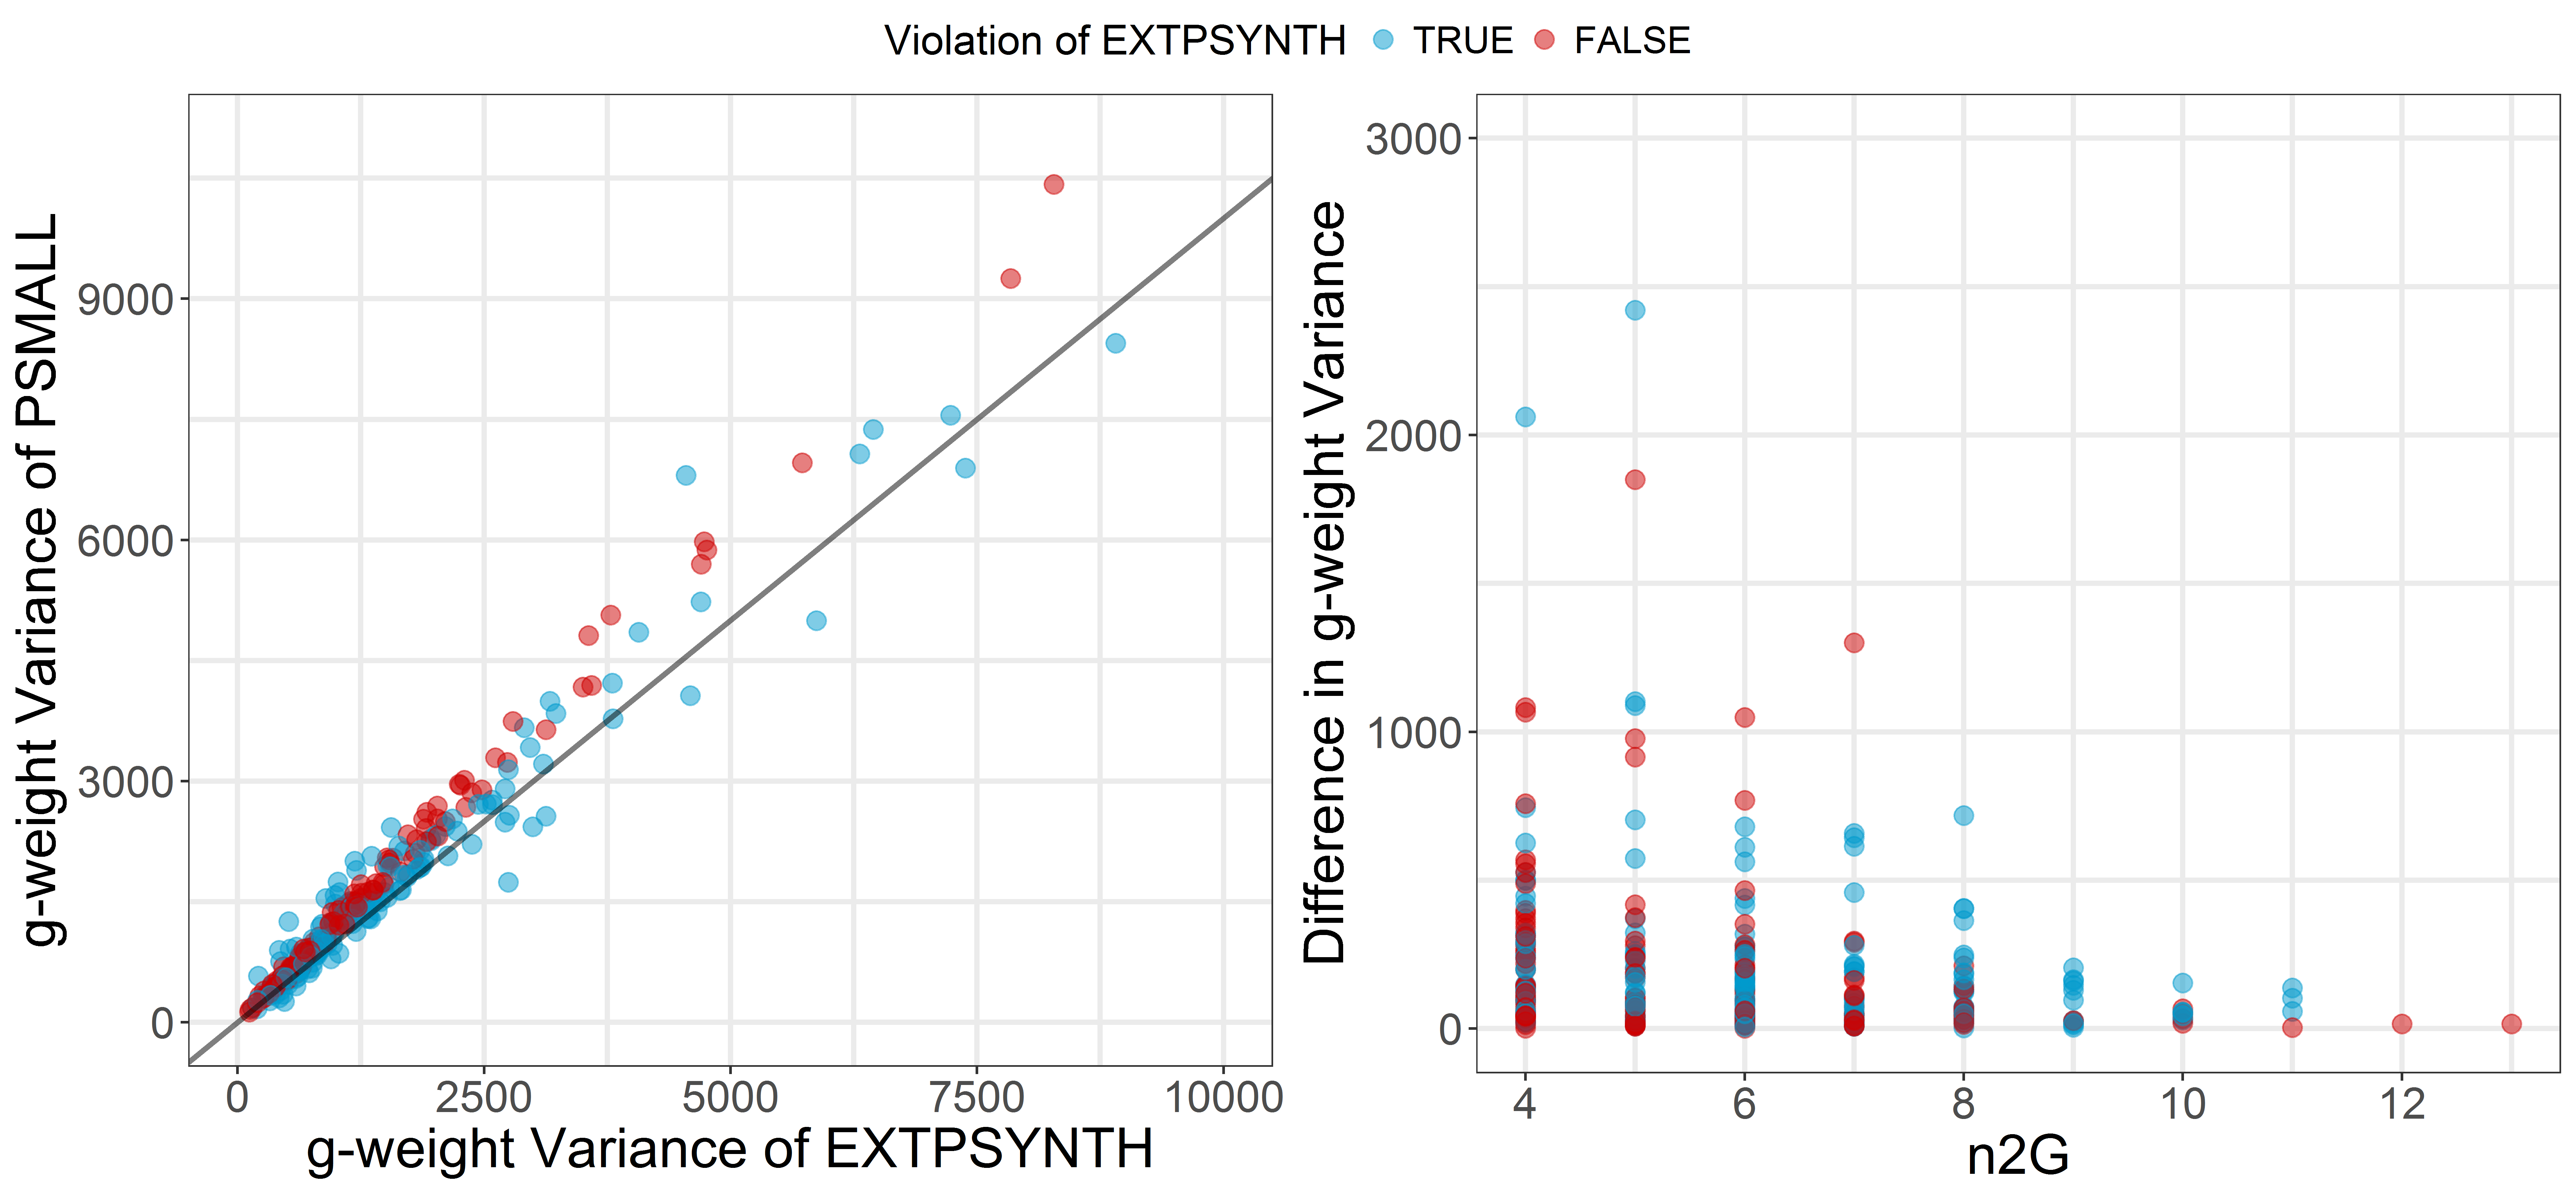
\includegraphics{fig/psmall_vs_extpsynth_fu.png}}
	\caption{\textit{Left}: Comparison of the g-weight variance between the PSMALL and the EXTPSYNTH estimator for the 321 FR units.
		      \textit{Right}: Difference in g-weight variance between the PSMALL and the EXTPSYNTH estimator in dependence of the terrestrial data ($n2G$) in the FR unit.}
	\label{fig:compvar}
\end{figure}








\newpage
% ----------------------------------------------------------------------- %
% ----------------------------------------------------------------------- %
\subsection{Effect of regression model accuracy}
\label{sec:modacc_eff}



















\begin{figure}[H]
	\centering
	\resizebox{1\hsize}{!}{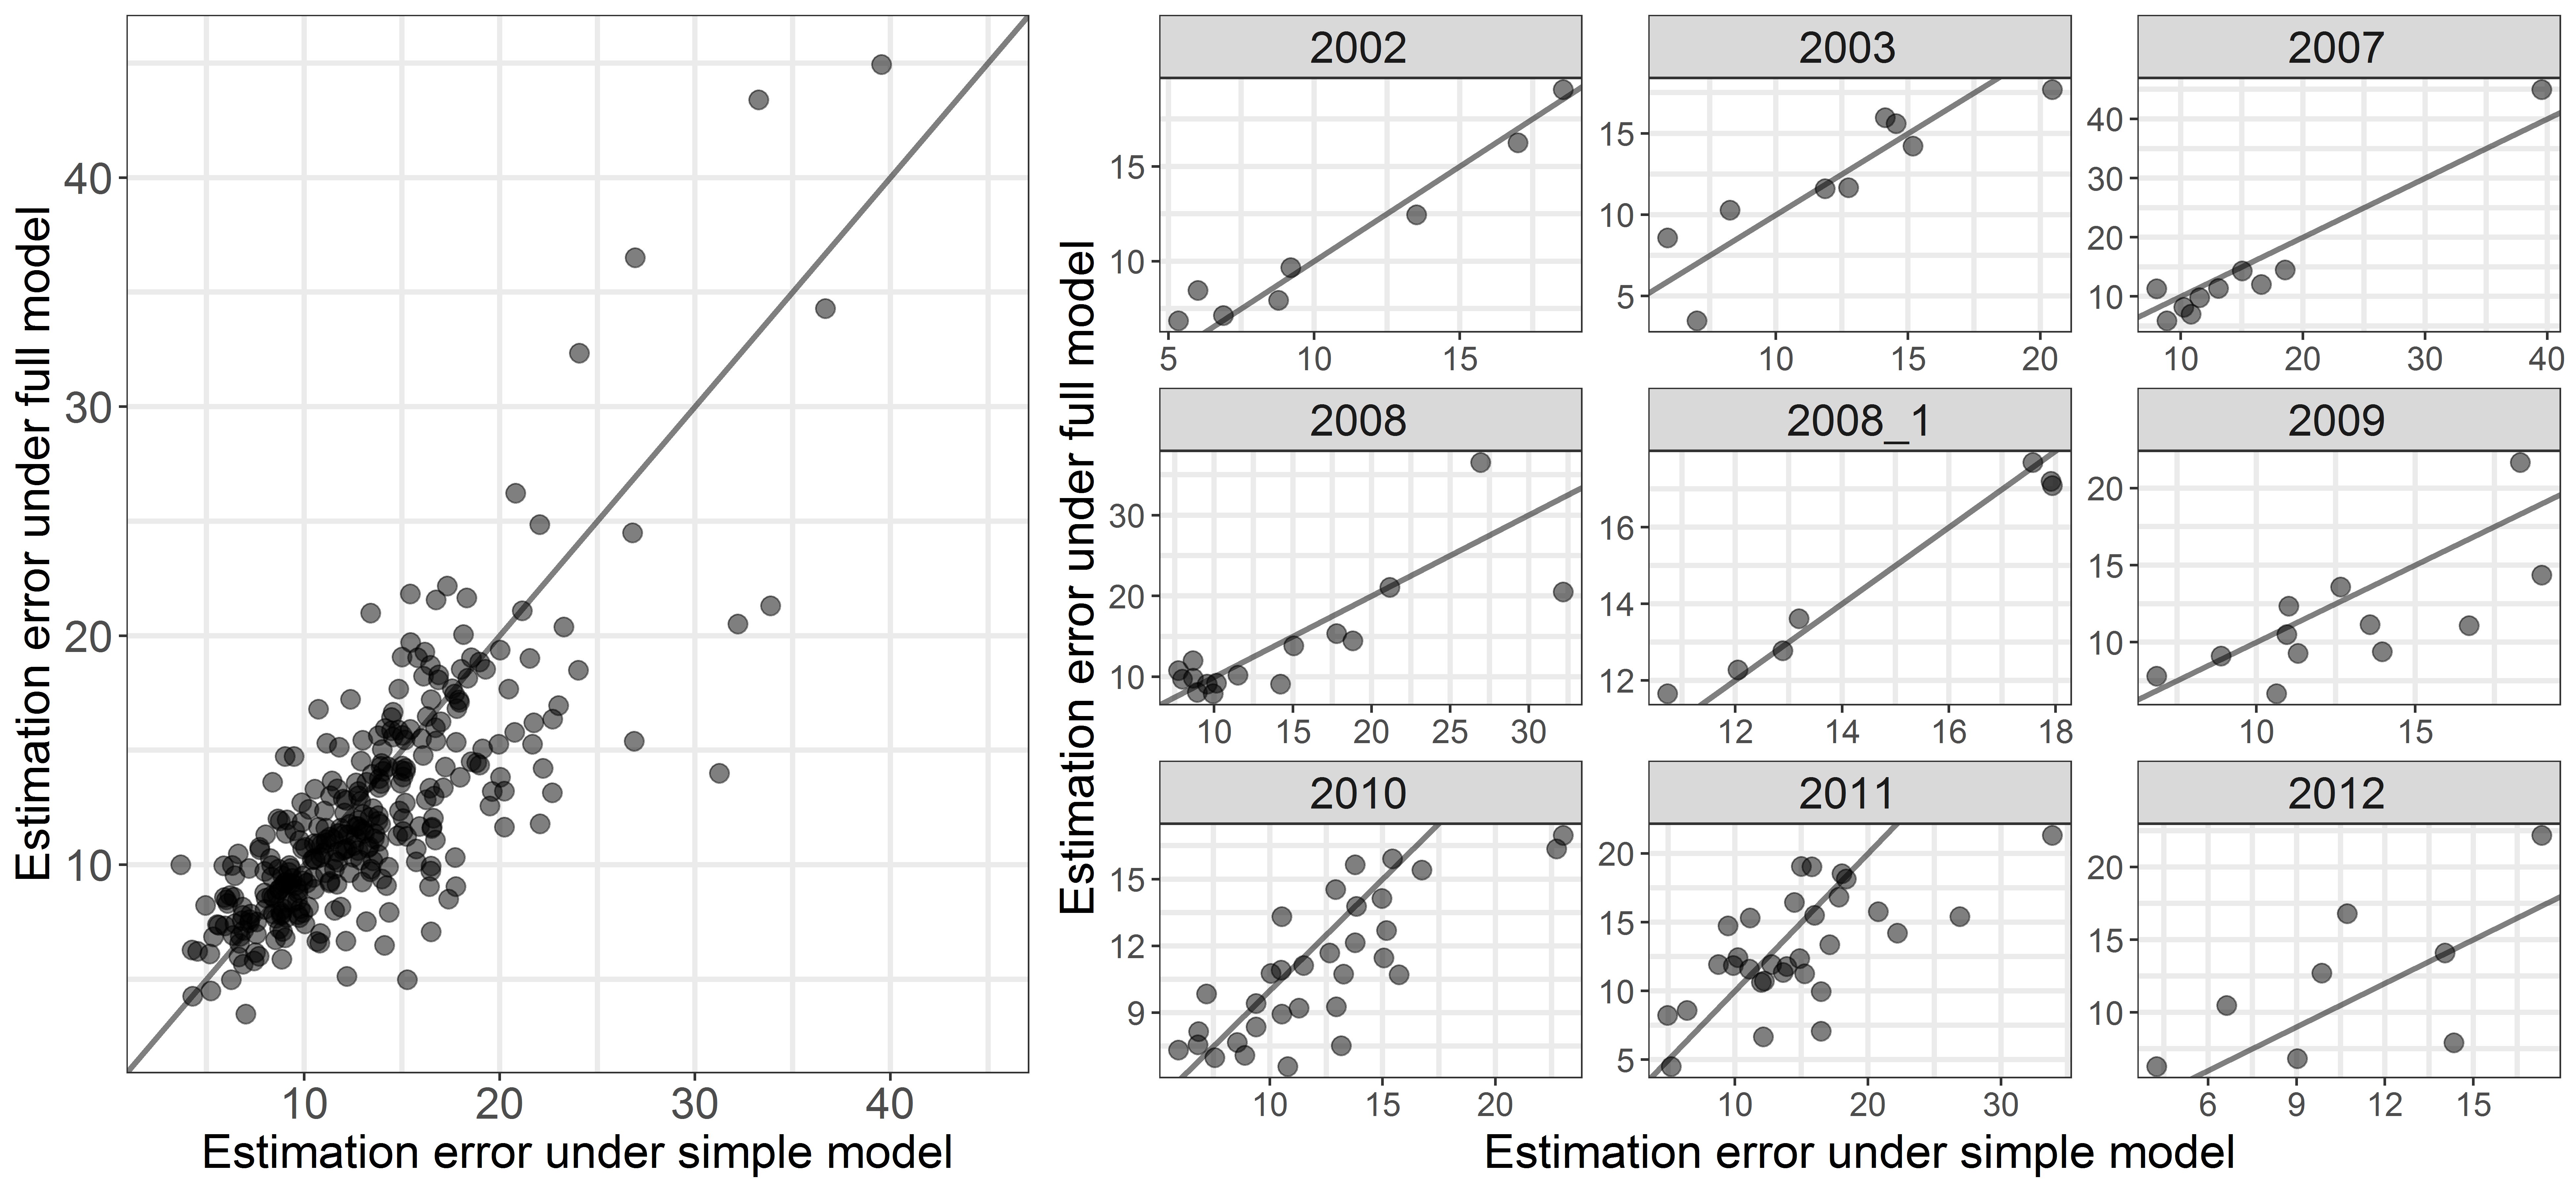
\includegraphics{fig/modcom_errors_fu.png}}
	\caption{}
	\label{fig:compmods}
\end{figure}





